\documentclass[usepdftitle=false,13pt]{beamer}

\usepackage{beamerthemesplit}

%\usepackage{beamerthemesplit} % need it?
%\usepackage{amsmath} % automatically included by beamer
\usepackage{amssymb} % no longer needed?
\usepackage{amsthm} % no longer needed?
\usepackage{amsfonts} % no longer needed?
\usepackage{graphicx} % automatically included by beamer?
\usepackage{verbatim} % useful for multi-line comments - collision?
%\usepackage{hyperref} % automatically included by beamer
\usepackage{url}

\usepackage{color}


\def\wl{\par \vspace{\baselineskip}}
%\usepackage[usenames,dvipsnames]{xcolor}
\usepackage{beamerthemesplit}
\usepackage{appendixnumberbeamer}



%\usepackage{algorithmic}
% greek support using xetex: compile with xelatex
% (other option: use latex with babel and greektex)
%\usepackage[cm-default]{fontspec} % [cm-default] is needed?
%\usepackage{xunicode}
\usepackage{hyperref}

\usepackage{appendixnumberbeamer}

\setbeamertemplate{bibliography item}[text]

%\usepackage{xltxtra}
%\usepackage{xgreek}
%\newcommand{\el}{\setlanguage{monogreek}}
%\newcommand{\en}{\setlanguage{american}}
%\newcommand{\eng}[1]{\setlanguage{american}#1\setlanguage{monogreek}}
\usepackage[absolute,overlay]{textpos}
\newcommand{\source}[1]{
\begin{textblock*}{4cm}(8.7cm,8.6cm)
    \begin{beamercolorbox}[ht=0.5cm,left,leftskip=2ex]{framesource}
        \usebeamerfont{framesource}\usebeamercolor[fg]{framesource} Source: {#1}
    \end{beamercolorbox}
\end{textblock*}
}

\setbeamercolor{framesource}{fg=gray}
\setbeamerfont{framesource}{size=\tiny}

\addtobeamertemplate{footnote}{\vspace{-6pt}}{\vspace{6pt}}

\renewcommand{\footnoterule}{}

\mode<handout>
{
  % handouts get a slight gray background to make frames noticeable
  \setbeamercolor{background canvas}{bg=black!5}
}


\mode<presentation>% or \mode<beamer>%?
{
  % main theme: specifies colors, fonts, inner and outer (all of these can be overwritten by subsequent commands)
  %\usetheme{Montpellier}
  %\usetheme{Warsaw}
  %\usetheme{Dresden}
  \usetheme{Singapore}

  %\usetheme[numbers,totalnumber,compress,sidebarshades]{PaloAlto}
  %\usetheme{Whale}
  %\usetheme[hideothersubsections,right,width=22mm]{Goettingen}

  % overwrite color theme if needed (there are inner, outer, inner+outer color themes):
  %\usecolortheme{seahorse}
  %\usecolortheme{beaver}
  \usecolortheme{seagull}
  %\usecolortheme{rose}
  % colors can also be specified directly for different parts of the frame:
  %\setbeamercolor{title}{fg=red!80!black,bg=red!20!white}
  %\setbeamertemplate{background canvas}[vertical shading][bottom=white,top=structure.fg!25]
  %\setbeamercolor{normal text}{bg=red!20} % gradient background?
  %\setbeamercolor{background canvas}{bg=} % for transparency

  % overwrite font theme, no actual font differences, just some options for presenting text:
  % invoke with a star to reset the size instead of accumulating
  %\usefonttheme[onlylarge]{structuresmallcapsserif}
  %\usefonttheme[onlylarge]{structurebold}
  %\usefonttheme[onlysmall]{structurebold}
  %\setbeamerfont{title}{shape=\itshape,family=\rmfamily}
  %\setbeamerfont*{frametitle}{size=\normalsize,series=\bfseries}

  % inner and outer themes can also be refined with \useinnertheme{themename} and \useoutertheme{themename}
  %\setbeamersize{text margin left=2em,text margin right=2em}
  %\setbeamersize{sidebar width left=1.5cm}
  %\setbeamersize{someMargin=someWidth} % to change margin sizes

  % other presentation options:
  % this will make invisible stuff not completely invisible:
  %\setbeamercovered{transparent}
  % uncover everything in a step-wise fashion:
  %\beamerdefaultoverlayspecification{<+->}
  % this will supress navigation symbols(?)
  %\setbeamertemplate{navigation symbols}{}
  %\setbeamertemplate{footline}[frame number]
}

  \makeatletter
  \beamer@theme@subsectiontrue 
  \makeatother
% χωρίς διάστημα στην αρχή των παραγράφων (μάλλον δεν χρειάζεται στο beamer)
%\setlength{\parindent}{0pt}
%\setlength{\parskip}{1ex plus 0.5ex minus 0.2ex}

% The table of contents will pop up at the beginning of each section:
\AtBeginSection[] % anything inside the [] will be displayed on section* instead - here nothing
{
  \begin{frame}<beamer>
    \frametitle{}
    \tableofcontents[currentsection]
  \end{frame}
}
% can also be used for subsections:
\begin{comment}
\AtBeginSubsection[] % anything inside the [] will be displayed on section* instead - here nothing
{
  \begin{frame}<beamer>
    \frametitle{}
    \tableofcontents[currentsection,currentsubsection]
  \end{frame}
}
\end{comment}
% other options for toc: pausesections, pausesubsections, currentsubsection, hideothersections, hideothersubsections

% At the start of each part, show an empty slide with the part name:
\AtBeginPart{\frame{\partpage}}


%%%%%%%%%%%%%%%% ΣΤΟΙΧΕΙΑ %%%%%%%%%%%%%%%%

% Τα στοιχεία πρέπει να δηλωθούν πριν αρχίσει το έγγραφο, ώστε να μπουν και στα στοιχεία του PDF

\title[CommunityCoin: a crypto currency for network communities]{CommunityCoin: a crypto currency for network communities}

\author[{p4u}]{p4u}
\institute[{guifi.net}]{guifi.net}
\date[\today]{\today}
%\date[\today]{\today}

% Δήλωση στοιχείων για το pdf
\hypersetup{
  pdftitle={a crypto currency for network communities},
  pdfauthor={p4u},
  pdfsubject={crypto currency},
  pdfkeywords={Commodity network, crypto currency}
}


% for authors with multiple affiliations:
%\author[Author, Another]{F.~Author\inst{1} \and S.~Another\inst{2}}
%\institute[Universities of Somewhere and Elsewhere]{
%  \inst{1} Department of Computer Science \\ University of Somewhere \and
%  \inst{2} Department of Theoretical Philosophy \\ University of Elsewhere
%}

% ορισμός logo: με includegraph ics (πακέτο graphics) ή pgfuseimage:
\pgfdeclareimage[height=1.0cm]{project-logo}{pic/logo}
\logo{\pgfuseimage{project-logo}}
%\logo{
\includegraphics[width=1.5cm]{figs/logo}}
%\titlegraphic{\pgfuseimage{university-logo}}
%\titlegraphic{\includegraphics[width=20mm]{upc.png}}




\begin{document}
\title[CommunityCoin\hspace{20em}\insertframenumber/\inserttotalframenumber]{CommunityCoin: a crypto currency for community networks}  
\author[p4u]{ p4u\\
 }

\date{\today} 

\frame{\titlepage}

%\section[Outline]{}
%\frame{\tableofcontents}



\section{Introduction}
\subsection{BitCoin}



\begin{frame}\frametitle{Proof of Work}
	\begin{itemize}
		\item Basic concept: a participant must proof some effort
		
		\item First used for preventing SPAM 
		
		\item Who wants to send an e-mail must include a hash with specific requirements
	
		\item It consumes CPU, so the e-mail sender must spend some time to send the text
	\end{itemize}
\end{frame}

\begin{frame}\frametitle{Proof of Work in BitCoin}
	\begin{itemize}
		\item BitCoin based on the same concept
		\item Currency transactions must be validated and included to a shared block chain
		\item The validation requires some work, so validators (miners) must spend resources
		\item There is a reward for the validation (this is how currency is generated)
	\end{itemize}
\end{frame}

\begin{frame}\frametitle{Bitcoin network}
The BitCoin network is a p2p network\\
Every peer needs to dowload the whole blockchain\\
Users use wallets as identifier: a set of asymetric keys\\
Users broadcast transactions which are validated by nodes (miners)\\
\begin{figure}[h!]
\begin{center}
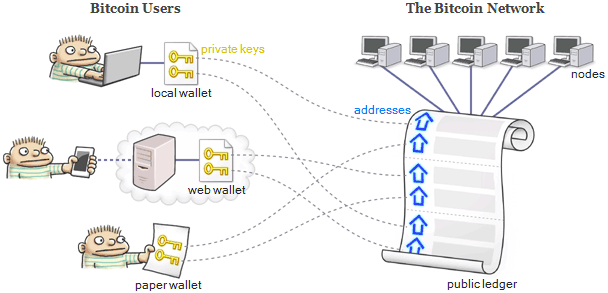
\includegraphics[width=0.45\textwidth]{pic/bitcoin-network}
\caption{BitCoin network}
\label{fig:block}
\end{center}
\end{figure}
\end{frame}

\subsection{BlockChain}

\begin{frame}\frametitle{Bitcoin block header}
A random set of pending transactions are collected.\\
Miner starts increasing Nonce and hashing the block header.\\
If the hash is smaller than the difficulty target, block is valid.\\
The difficulty target is calculated every 2016 blocks\\
\begin{figure}[h!]
\begin{center}
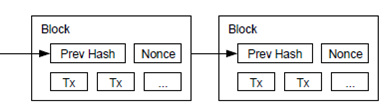
\includegraphics[width=0.45\textwidth]{pic/block}
\caption{Blockchain header}
\label{fig:block}
\end{center}
\end{figure}
\end{frame}

\begin{frame}\frametitle{BlockChain}
	As you can guess, the blockchain can be used for many purposes
	\begin{itemize}
		\item A distributed domain name system (NameCoin)
		\item A platform to sign legal documents
		\item A platform to validate that a photo has been taken in a specific time
		\item A voting system
		\item etc...
	\end{itemize}
	It is just fucking amazing!
\end{frame}



\section{CommunityCoin}

\subsection{Motivation}

\begin{frame}\frametitle{Motivation}
	\begin{itemize}
		\item Community is not only about tech stuff, it involves also social-economic aspects
		\item We own our network, why not to own our own economic system?
		\item It adds many new ways for funding thus it makes the community more sustenible
		\item It might incentivate community users to work for the community
		\item It can be fun :)
	\end{itemize}
\end{frame}





\frame{\titlepage}

\end{document}
